%%%%%%%%%%%%%%%%%%%%%%%%%%%%%%%%%%%%%%%%%
% Short Sectioned Assignment
% LaTeX Template
% Version 1.0 (5/5/12)
%
% This template has been downloaded from:
% http://www.LaTeXTemplates.com
%
% Original author:
% Frits Wenneker (http://www.howtotex.com)
%
% License:
% CC BY-NC-SA 3.0 (http://creativecommons.org/licenses/by-nc-sa/3.0/)
%
%%%%%%%%%%%%%%%%%%%%%%%%%%%%%%%%%%%%%%%%%

%----------------------------------------------------------------------------------------
%	PACKAGES AND OTHER DOCUMENT CONFIGURATIONS
%----------------------------------------------------------------------------------------

\documentclass[paper=a4, fontsize=11pt]{scrartcl} % A4 paper and 11pt font size

\usepackage[T1]{fontenc} % Use 8-bit encoding that has 256 glyphs
%\usepackage{fourier} % Use the Adobe Utopia font for the document - comment this line to return to the LaTeX default
\usepackage[english]{babel} % English language/hyphenation
\usepackage{amsmath,amsfonts,amsthm} % Math packages

\usepackage{lipsum} % Used for inserting dummy 'Lorem ipsum' text into the template

\usepackage{sectsty} % Allows customizing section commands
\allsectionsfont{ \normalfont\scshape} % Make all sections centered, the default font and small caps

\usepackage{graphicx}
\usepackage{booktabs}
\usepackage[framed,numbered,autolinebreaks,useliterate]{mcode}

\usepackage{fancyhdr} % Custom headers and footers
\pagestyle{fancyplain} % Makes all pages in the document conform to the custom headers and footers
\fancyhead{} % No page header - if you want one, create it in the same way as the footers below
\fancyfoot[L]{} % Empty left footer
\fancyfoot[C]{} % Empty center footer
\fancyfoot[R]{\thepage} % Page numbering for right footer
\renewcommand{\headrulewidth}{0pt} % Remove header underlines
\renewcommand{\footrulewidth}{0pt} % Remove footer underlines
\setlength{\headheight}{13.6pt} % Customize the height of the header

\numberwithin{equation}{section} % Number equations within sections (i.e. 1.1, 1.2, 2.1, 2.2 instead of 1, 2, 3, 4)
\numberwithin{figure}{section} % Number figures within sections (i.e. 1.1, 1.2, 2.1, 2.2 instead of 1, 2, 3, 4)
\numberwithin{table}{section} % Number tables within sections (i.e. 1.1, 1.2, 2.1, 2.2 instead of 1, 2, 3, 4)

\setlength\parindent{0pt} % Removes all indentation from paragraphs - comment this line for an assignment with lots of text

%----------------------------------------------------------------------------------------
%	TITLE SECTION
%----------------------------------------------------------------------------------------

\newcommand{\horrule}[1]{\rule{\linewidth}{#1}} % Create horizontal rule command with 1 argument of height

\title{	
\normalfont \normalsize 
\textsc{APSC 1001, George Washington University} \\ [25pt] % Your university, school and/or department name(s)
\horrule{0.5pt} \\[0.4cm] % Thin top horizontal rule
\huge APSC 1001 Introduction to Matlab \#2 \\ % The assignment title
\horrule{2pt} \\[0.5cm] % Thick bottom horizontal rule
}

\author{\normalsize Based on "Getting Your Hands Dirty With MATLAB by Dr. Kartik Bulusu } % Your name

%\normalsize Week 1 Handout
\date{\normalsize \today } % Today's date or a custom date


\begin{document}

\maketitle % Print the title

\section{Matrices in MATLAB}

MATLAB assumes every variable to be potentially, a matrix. Recalling the definition of an array we can start creating matrices in MATLAB.\\

An array is a list of numbers or expressions arranged in horizontal rows and vertical columns. When an array has one row or column, it is called a vector. An array with $m$ rows and $n$ columns is a called a matrix of size $m \times n$. (Pratap, 1999)\\

A matrix is entered row-wise, the rows separated by semicolons or carriage returns. Elements of the matrix may be real or complex numbers, or valid MATLAB expressions.

\begin{center}
	\begin{tabular}{ c c }
	\toprule
	\textbf{Matrix} & \textbf{MATLAB input command}\\
	\midrule\\
	\addlinespace[-2ex]
	$A = \begin{bmatrix}  1 & 2 & 7 \\ 4 & 9 & 0 \end{bmatrix}$ &
	$A = [1\ 2\ 7; 4\ 9\ 0]$\\
	\addlinespace[1.5ex]
	$B = \begin{bmatrix}  8x & ln(x)+sin(y)\\ 3i & 7+2i \end{bmatrix}$ &
	$B = [8*x\ log(x)+sin(y); 3i\ 7+2i]$\\
	\bottomrule
	\end{tabular}
\end{center}

\subsection{Vectors and Scalars as special cases of matrices}
	
\begin{itemize}
	\item A \textit{vector} is a special case of a matrix, with just one row or one coulmn.
	It is entered the same way as a matrix.
	
	$>>x = [1\ 5\ 9];$ \hspace{.2\textwidth}\% produces a row vector
	
	$>>y = [1; 5; 9]; $ \hspace{.2\textwidth}\% produces a column vector
	
	\item A \textit{scalar} can be thought of as a matrix with just one row and one column.
	A scalar does not require brackets when entered.
	
	$>>g = 9.81;$ \hspace{.15\textwidth}\% notice that the semicolon suppresses the output
	
	\item A \textit{null} or empty matrix has no elements in it. Create a null matrix with square brackets. This can be useful for initializing matrices, although it is not necessary every time.
	
	$>>u=[\ ];$
\end{itemize}

\subsection{Indexing Matrices}

Once a matrix is created in MATLAB, it's elements can be accessed by specifying the index of their
row and column.\\

A(i,j) in MATLAB refers to the element in the \textit{i}th row and \textit{j}th column of a matrix A. 
While this notation is fairly common in many programming languages, MATLAB provides a few more options in index specification.
These options make matrix manipulation much easier than in other programming languages.

\begin{itemize}
	\item A(m:n, k:l) specifies rows \textit{m} to \textit{n} and columns \textit{k} to \textit{l} of matrix A.
	\item A(:, 3:6) refers to columns 3 through 6 of all rows (:) in matrix A.
\end{itemize}

\textbf{Walk through these examples on your own.} You should type each example and make sure you understand what is happening and why it happens. These are the basics of MATLAB; learning them now is the only way we can cover more advanced topics this semester.\\

\begin{verbatim}
>> A = [1 2 3; 4 5 6; 7 8 8] %Matrices are entered row-wise. Rows are 
%separated by semicolons and columns are separated by spaces or commas.

A =
 1 2 3
 4 5 6
 7 8 8

>> A(3,2)	%Element A(3,2) is accessed
ans =
 8
 
>> A(3,3) = 9	%Changing an element in matrix A
A =
 1 2 3
 4 5 6
 7 8 9
 
>> B = A(2:3, 1:3)	%Any submatrix of A is generated by specifying the range 
%of rows and columns
B = 
 4 5 6
 7 8 9
 
>> B = A(2:3, :) %All rows or all columns of a matrix
%can be accessed by specifying ':' as the index 
B = 
 4 5 6
 7 8 9
 
>>B(:,2) = [ ]	%A row or column of a matrix is 
%deleted by setting it to a null vector
B = 
 4 6
 7 9

\end{verbatim}

\section{Matrix Manipulation and Operations}

We have already seen that it is easy fairly easy to correct wrong entries, add or delete rows or
columns or extract a submatrix from a matrix because of the unique indexing feature in MATLAB.
Matrix dimensions are determined automatically by MATLAB.
In order for MATLAB to be useful, we need to perform matrix operations on the matrices we have created.

\begin{itemize}
\item \textbf{Matrix Algebra} is different from element-by-element arithmetic. 
\begin{itemize}
\item Matrix addition and subtraction only work if the matrices are of identical size. 

\item Matrix multiplication is valid if the number of columns in A equals the number of rows in B.

\item Scalar multiplication takes a single value and multiplies it by each entry in a matrix. 
This is written the same way as matrix multiplication, $\alpha \cdot A$, but has a very different result.

\item Matrix division can be a tricky topic. 
In MATLAB A/B is equivalent to $A\cdot B^{-1}$, and $A \textbackslash B$ is equivalent to $A^{-1}\cdot B$. 
\item Neither matrix multiplication nor division is commutative.

\item Matrix powers are only valid for square matrices.
$A^2$ is equivalent to $A \cdot A$.
In a linear algebra class you may discuss these topics further. 
\end{itemize}

\item \textbf{Element by element operations} use the operator '.' in MATLAB. 
Using this operator, you can multiply each term in a vector by one term in another vector.
See the examples for further information.

\item \textbf{Other common matrix operations}
	\begin{itemize}
	\item The \textit{transpose} operator, $A'$, switches the rows and columns of A
	\item The \textit{exponent} operator, .\^\ , raises each element in an array to an exponent
	\item \textbf{size(A)} returns the number of rows and columns in a matrix
	\item \textbf{det(A)} takes the \textit{determinant} of matrix A
	\item \textbf{max(v)} and \textbf{min(v)} give the maximum and minimum entries in a vector, respectively
	
	\end{itemize}

\item \textbf{Utility Matrices}

To further aid matrix manipulation and creation, MATLAB provides some useful utility matrices. 
\begin{itemize}
	\item \textbf{eye(m,n)} returns an \textit{m} by \textit{n} matrix with 1's on the main diagonal, also called the \textit{identity} matrix
	\item \textbf{zeros(m,n)} returns an \textit{m} by \textit{n} matrix with all zeros
	\item \textbf{ones(m,n)} returns an \textit{m} by \textit{n} matrix with all ones
	\item \textbf{rand(m,n)} returns an \textit{m} by \textit{n} matrix of random numbers between 0 and 1
	\item \textbf{diag(v)} creates a matrix with vector \textbf{v} on the main diagonal
	\item \textbf{diag(A)} creates a vector of the main diagonal of matrix A
\end{itemize}
\end{itemize}

\subsection{Examples}

\begin{verbatim}
>>A = [1 2 3; 2 3 4; 6 4 8];
>>B = [2 3 4; 2 5 7; 9 3 2];
>>C = A*B %Notice the different outputs of A*B vs A.*B 
C = 
 33 22 24
 46 33 37
 92 62 68
 
>>D = A.*B
D = 
 2  6 12
 4 15 28
 54 12 16
 
>>E = A\B
E = 
  0.1667 -0.1667 -0.3333
 -2.3333  3.3333  5.6667
  2.1667 -1.1667 -2.3333

>>F = inv(A)*B	 %The result of this is identical to the previous example
F =     	
  0.1667 -0.1667 -0.3333
 -2.3333  3.3333  5.6667
  2.1667 -1.1667 -2.3333 	

>>A = [1 5 3; 4 2 6];
>>size(A)
ans = 
 2 3
 
>>[m, n] = size(A)  %answers returned by a function can be saved as variables.
m = 
 2
n = 
 3
 
>>A' 	%transpose operator
ans = 
 1 4
 5 2
 3 6
 
>>eye(3)
ans = 
 1 0 0
 0 1 0
 0 0 1
 
>>[max_value, max_index] = max(A)
max_value = 
 4 5 6
max_index = 
 2 1 2

\end{verbatim}
\newpage
\section{Plotting}
\subsection{Useful Functions}
There are a few functions that are in MATLAB which are not specific to plotting, but will be both helpful and frequently used.

\begin{itemize}
\item \textbf{help \textit{function}} In the MATLAB command window, you can type \textit{help} then the name of any function. This will bring up documentation on the different uses for that function, the arguments it takes, what it returns, and often example uses and related functions. Further help and documentation is available online, or by typing \textit{doc} plus the name of the function. 
\item \textbf{linspace(m,n,N)} The linspace function creates an array of size $m \times n$ with $N$ linearly spaced entries.
\begin{verbatim}
>>t = linspace(0, 1, 11) %notice that 11 numbers are required to create 10 steps between 0 and 1 
t =
  Columns 1 through 7
         0    0.1000    0.2000    0.3000    0.4000    0.5000    0.6000

  Columns 8 through 11
    0.7000    0.8000    0.9000    1.0000
\end{verbatim} 
 
\item \textbf{colon operator}	The colon, :, is used in Matlab to denote ranges of numbers. It can also be used to create arrays. The command:
\begin{verbatim}
>>t = 0:0.1:1	
\end{verbatim} 
will create an array with entries ranging from 0 to 1 in step sizes of 0.1. 
This will have the same output as the previous \textit{linspace(m, n, N)} example
\end{itemize}

\subsection{Plot Command}
The plot command in MATLAB looks like the following: 
\mcode{plot(x, y, optional_arguments)}
In order to plot arrays in Matlab, they must be of the same length.
The optional arguments cover settings on the figure such as labels, color, or style. 
Type 'help plot' for more information.\\

The best way to learn how the plot functionality in MATLAB works is with an example.
\newpage
\lstinputlisting[firstline=4,lastline=15]{plotting_examples.m}
The code above will produce the following output: 
\begin{figure}[h!]
\centering
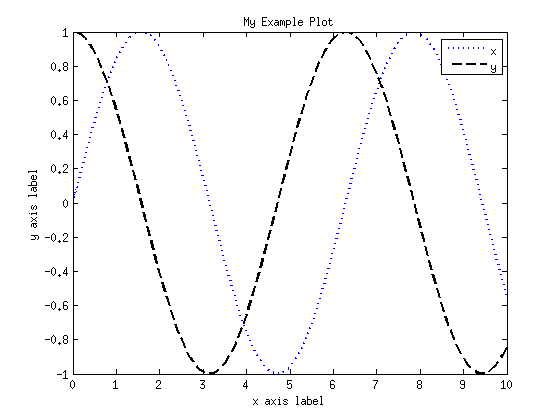
\includegraphics[scale=.75]{plot_example}
\caption{It is good practice (and required for this class!) to always include a title and axis labels for each plot.}
\end{figure}
The figure will open in a new window. Multiple figure windows can be open at a time, and any plotting commands will affect the current figure, which is the most recently selected figure window. Unless the \textit{hold} option is on, a plot command will overwrite an existing plot.
\subsection{Additional Commands}
Some useful commands for plotting can be found below. For more information, use the help function.
\begin{itemize}
\item The \mcode{figure} command will open a new figure window. With an argument, \mcode{figure(1)} will open a specific existing figure window.
\item The command \mcode{close} will close the current figure window.
\mcode{close all} will close all open figures.
\item A useful property of a figure window is its hold state, which determines whether an additional \mcode{plot} command will overwrite the current figure or add to it. 
The command \mcode{hold on} or \mcode{hold off} will change this state. 
\item MATLAB will automatically scale the axes of a plot. To set them manually, use the \mcode{axis({xmin xmax ymin ymax]}} command.
\item To create a legend for your figure, use the \mcode{legend('string one', 'string two'} command.

\end{itemize}

\newpage
\section*{\textbf{References}}
[1] Pratap, R., \textit{Getting Started with MATLAB 5 - A Quick Introduction for Scientists and Engi-
neers}, Oxford University Press, 1999.\\

[2] Kreyszig, E., \textit{Advanced Engineering Mathematics}, 8th ed., John Wiley \& Sons, Inc., 1999.



%----------------------------------------------------------------------------------------

\end{document}